\subsection{Android Application Package} \label{subsection:foundation-android-package}
Android applications are distributed and installed using the \gls{apk} file format.
The \gls{apk} format is based on the ZIP file archive format and contains the code and resources of the application.
They can be installed using different mechanisms.
The prefered and most secure is the installation from the Google Play Store.
It provides the \gls{apk} from a trusted source and installs it automatically.
Other application stores provide the \gls{apk} from a trusted source and facilitate the manual installation.
Yet another application stores are less trusted.
In addition, the \gls{apk} can be obtained from anywhere and installed manually.
\newline
The build process of \gls{apk} contains several steps which are visualized in figure~\ref{fig:apk}.
\newline
\begin{figure}[h]
    \centering
    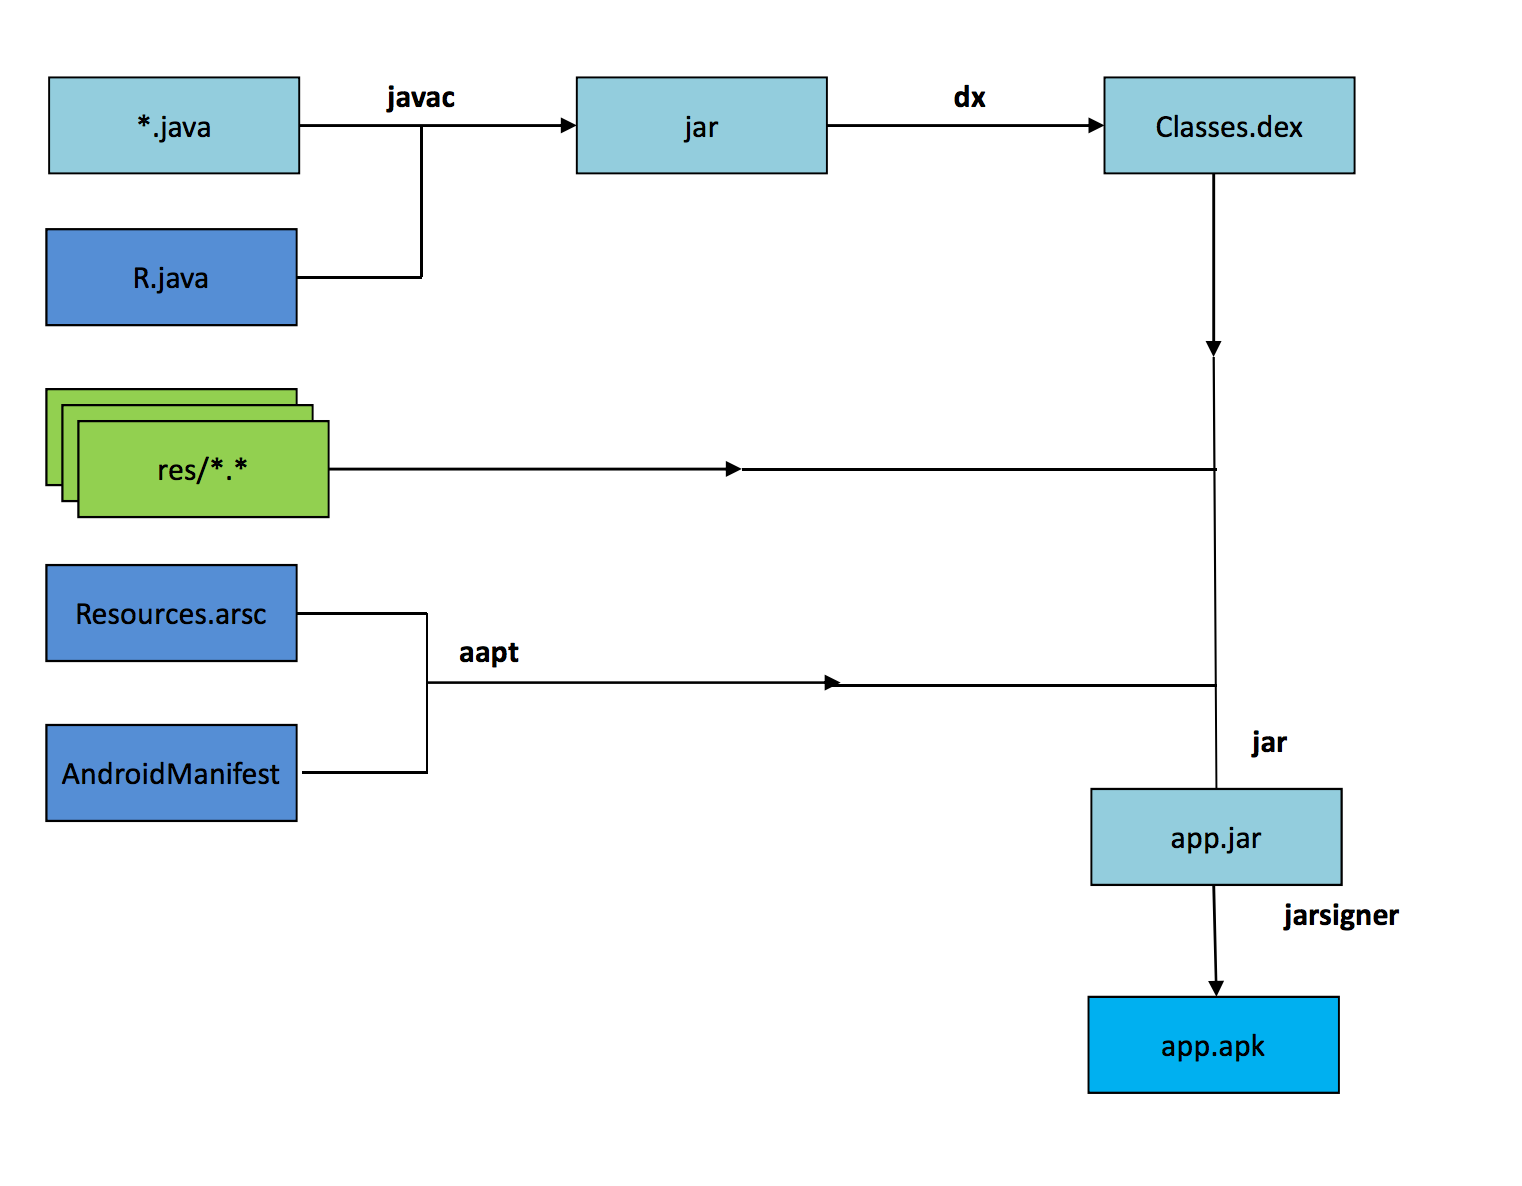
\includegraphics[width=0.8\textwidth]{data/apk.png}
    \caption{\gls{apk} build process \cite{andevconDalvikART}}
    \label{fig:apk}
\end{figure}
Since Android applications are usually written in Java, there are similarities to the Java program build process.
Upon compilation, the source code is transformed into \gls{classg} files by the Java Compiler javac.
Each Java class is stored as bytecode in the corresponding \gls{classg} file.
Java bytecode can recompiled to become readable.
To prevent that, obfuscation can be applied as described in section~\ref{subsection:counter-improve-obfuscation}.
When all Java classes are compiled to \gls{classg} files, they are packed into a \gls{jar} file.
\newline
Android uses a \gls{vm} different from Java.
It requires the Java bytecode to be converted to a different format - the Dalvik bytecode.
The Android \gls{sdk} provides \textit{dx}, the tool used to convert \gls{classg} files to a single \textit{classes.dex} file.
The \gls{vm} and the \gls{dex} file format will be described in the following.
\newline
The \gls{apk} itself consists of three parts.
\begin{itemize}
\item \textit{classes.dex}, a file containing the bytecode
\item resource files (\textit{res/*.*}), a directory containing static content like images, the strings.xml and the layout.xml files
\item \textit{Resources.arsc}, containing compiled resources, and \textit{AndroidManifest.xml}, containing essential information like required permissions
\end{itemize}
The \textit{apkBuilder} combines these files into one archive file, which is signed and zipaligned to become a valid \gls{apk}.
The \textit{jarsigner} uses the developer’s private key to sign the application similar to the Java code signing \cite{codeSigning}.
This signing process ensures integrity and authenticity using a self-signed certificate, i.e. it provides a key usable to decrypt and authenticates the entity it claims to comes from.
As there is no certificate authority (CA), this entity cannot be linked, trusted or not, to a person or entity in the real world.
Upon update the entities previous and current version can be compared and the update prevented on mismatch. \cite{nelenkovSelf}
Afterwards \textit{zipalign} is used to mark uncompressed data. \cite{androidPublishSign} \cite{androidSigning} \cite{andevconDalvikART}
\newline
\newline
The structure of a final \gls{apk} file has the following content as minimum as seen in figure~\ref{fig:apkfolder}.
\begin{figure}[h]
    \centering
    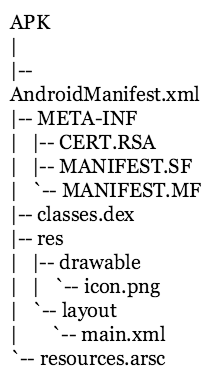
\includegraphics[width=0.5\textwidth]{data/apkfolder.png}
    \caption{\gls{apk} folder structure}
    \label{fig:apkfolder}
\end{figure}
The \textit{AndroidManifest.xml} and the \textit{classes.dex} have already been covered.
\newline
The \gls{apk} has the same code signing mechanism as Java .
The \textit{META-INF} folder is used to store the signing information, e.g. the manifest and certificate. \cite{codeSigning} \cite{metaJava}
\newline
While the static resources, like drawables and layouts, are in the res folder, the resources.arsc contains the compiled resources.
\newline
Native libraries are written in C or C++ in order to boost performance and allow low level interaction between applications and the kernel by using the \gls{jni}.
They are stored as \textit{*.so} files in the libs folder, sorted by their specific architecture, like armeabi-v7a for ARM or x86 for Intel processors.
\cite{kovachevaMaster} \cite{ehringerDalvik}
